\chapter{SIPOC Analysis}

The SIPOC diagram provides a high-level overview of the Coffee Chain ERP process, highlighting how Suppliers, Inputs, Processes, Outputs, and Customers interact. It is a useful tool for understanding the flow of operations, identifying bottlenecks, and ensuring that all stakeholders’ needs are addressed.

\section*{Purpose of SIPOC}
The SIPOC framework helps us visualize the end-to-end process of the Coffee Chain ERP system. It allows management to:
\begin{itemize}
    \item Identify key suppliers and inputs required for smooth operations.
    \item Understand the critical processes that transform inputs into outputs.
    \item Ensure outputs meet the expectations of customers.
    \item Detect potential gaps or inefficiencies in the workflow.
\end{itemize}

\section*{Suppliers, Inputs, Processes, Outputs, Customers}

\subsection*{Suppliers}
\begin{itemize}
    \item \textbf{Coffee Outlets:} Provide sales data, menu updates, and operational feedback. They are the primary source of information for the ERP system.
    \item \textbf{Suppliers:} Supply raw ingredients, coffee beans, and other consumables. Timely delivery ensures smooth operations across outlets.
    \item \textbf{CRM:} Provides customer leads and engagement data, which is essential for marketing and sales tracking.
\end{itemize}

\subsection*{Inputs}
\begin{itemize}
    \item Product details, pricing, and menu configurations.
    \item Raw materials and stock updates from suppliers.
    \item Customer leads and engagement information from the CRM.
\end{itemize}

\subsection*{Processes}
\begin{itemize}
    \item Tracking daily sales and updating the ERP system.
    \item Managing product and menu updates in real-time.
    \item Receiving and logging stock from suppliers.
    \item Capturing customer interactions and monitoring CRM data.
\end{itemize}

\subsection*{Outputs}
\begin{itemize}
    \item Updated sales reports for each outlet and consolidated regional reports.
    \item Inventory reports and notifications for low-stock items.
    \item Real-time product updates for sales and POS systems.
    \item CRM insights for marketing and customer engagement.
\end{itemize}

\subsection*{Customers}
\begin{itemize}
    \item Management: Receives comprehensive reports for decision-making.
    \item Outlet Managers: Use outputs to manage day-to-day operations.
    \item Marketing/Sales Teams: Leverage CRM insights to plan campaigns.
    \item Customers: Benefit indirectly through accurate pricing, better product availability, and consistent service.
\end{itemize}

\section*{SIPOC Table}

\begin{table}[H]
\centering
\begin{tabular}{|p{3cm}|p{3cm}|p{4cm}|p{3cm}|p{3cm}|}
\hline
\textbf{Suppliers} & \textbf{Inputs} & \textbf{Process} & \textbf{Outputs} & \textbf{Customers} \\
\hline
Coffee outlets & Product & Track sales, update ERP, manage orders & Sales reports, product updates & Management, Customers \\
\hline
Suppliers & Ingredients, stock & Receive and log stock in ERP & Updated inventory & Outlet managers, Kitchen staff \\
\hline
CRM & Customer leads & Capture and manage leads & Lead reports, CRM data & Marketing, Sales team \\
\hline
\end{tabular}
\caption{SIPOC for Coffee Chain ERP}
\end{table}

\section*{Visual SIPOC Diagram}

\begin{figure}[H]
\centering
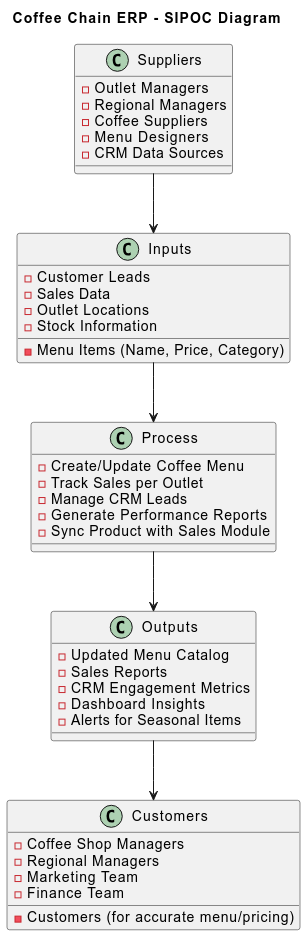
\includegraphics[width=0.85\textwidth,height=0.6\textheight,keepaspectratio]{diagrams/SIPOC.png}
\caption{Visual SIPOC Diagram of Coffee Chain ERP}
\end{figure}

\section*{Insights}
The SIPOC analysis highlights:
\begin{itemize}
    \item Critical dependency on real-time data from outlets and suppliers.
    \item Integration points between menu, sales, and CRM that require automated updates.
    \item The need for dashboards to provide management with actionable insights.
    \item Potential bottlenecks such as delayed supplier updates or manual sales entry.
\end{itemize}
